\subsection{Accuracy Evaluation}
\label{sec:results_gocard}
%
We present now our results on the GoCard database for all aggregate functions \texttt{count, sum, avg, min, max}. 
%
Hence, the view space $SP = 5 \times 9 \times 3 = 135$ views.
%
Similar to the previous experiments, we used Earth Movers Distance (EMD) as the deviation metric for computing the utility of a view.
%
%The dataset used is $GoCard$. 
%we run this experiment on over \emph{All} aggregate functions \emph{Count, Sum, Average, Min, and Max} 
%space size GoCard =$5 \times 9 \times 3=135$ views and the deviation metric is Earth Movers Distance (EMD). \\ %\mas{what is the input query(s)?} 
Also, we use the following query as our target view:
%
\begin{center}
\texttt{$Q:$ SELECT * FROM GoCard WHERE alightingstop ='University of Queensland';}
\end{center}
%
%\thefontsize 
%\mas{use straight lines to connect points not curves}
%\mas{use the right accuracy metric}
%

Figure \ref{fig:fig1} shows the accuracy of the results produced by algorithms $Sela$, $Diff DVal$, $DimHisto$ and $SeeDB Rnd$ to find Top-$25$ views comparing with different view space $R$ values. 
%
As shown, the proposed algorithms $Sela$ and $Diff DVal$ scored the same accuracy in the first 30 explored views. 
%
However, $DimsHisto$ shows lower accuracy than $Sela$ and $Diff DVal$ when the number of explored views is 45. 
%
The reason is, $DimHisto$ evaluates dimension attributes according to their frequencies, hence, it is less descriptive to some aggregate functions such as \texttt{max, min}.  
%
Note that the accuracy of the proposed algorithms increases with $R$, as shown in Figure \ref{fig:fig1}.
%\mas{so why it is not doing better when supposedly you proposed it to improve on the first one}
Finally, $SeeDB Rnd$ obtains the lowest accuracy while varying $R$, except when it considers almost all the views, i.e., when $R$ approaches $SP$. 
%

\begin{figure}[t]
  \centering
%\end{figure}
  \begin{subfigure}[b]{0.42\textwidth}
    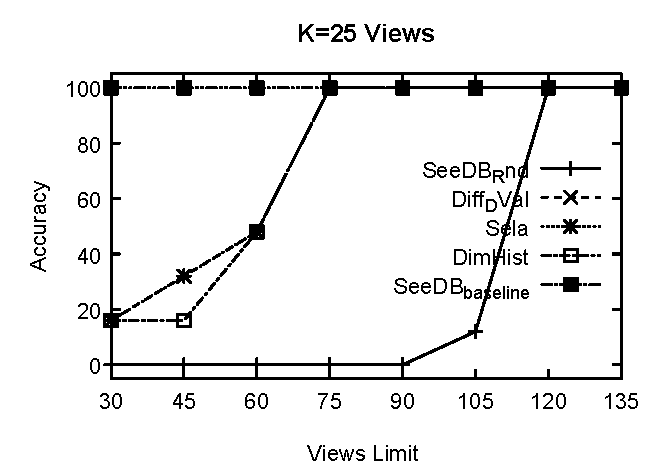
\includegraphics[width=\textwidth]{21.pdf}
    \caption{Accuracy}
        \label{fig:fig1}%
  \end{subfigure}
  %
  \begin{subfigure}[b]{0.42\textwidth}
    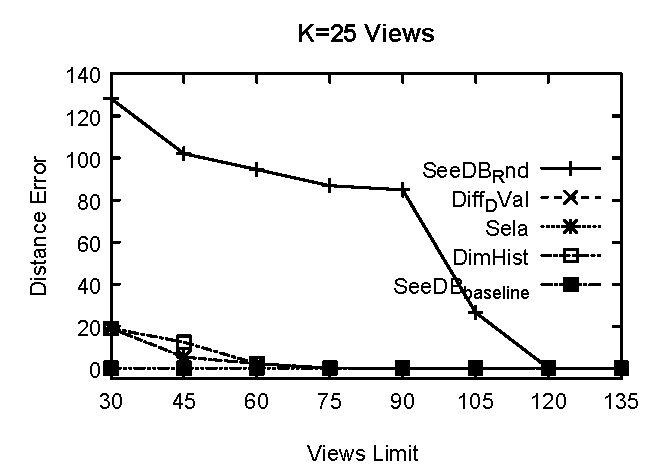
\includegraphics[width=\textwidth]{22.pdf}
     \caption{Distance error}
        \label{fig:figa2}
  \end{subfigure}
  \caption{Results quality while varying view space $R$ and $K = 25$}
\end{figure}

 %\begin{figure}[h]
%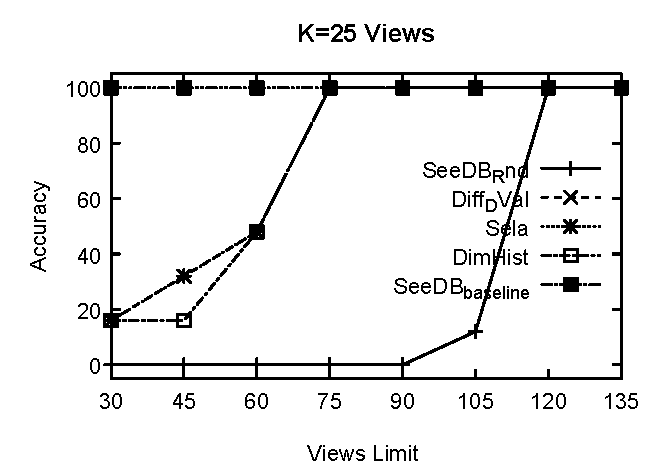
\includegraphics[width=\textwidth]{21.pdf}
%\caption{Accuracy compared with  the view space size for the Algorithms $Sela$ , $N-N'$, $DimHisto$, and $SeeDB_Rnd$}
%\label{fig:fig1}%
%\end{figure}

%\mas{use lines for all and only one y-axis}
Figure \ref{fig:figa2} reports the distance error produced by algorithms $Sela$, $Diff DVal$, and $DimsHisto$ to find Top-25 $(K=25)$ views across different values of $R$. 
%
As shown, our proposed algorithms succeed to minimize the distance error as quickly as $SeeDB Baseline$, especially when expanding the space size $R$. 
%
Although algorithm $DimsHisto$ obtains lower accuracy than $Sela$ and $Diff DVal$ as shown in Figure \ref{fig:fig1} when $R = 45$, the distance error at the same view space is low. 
%
This is because $DimsHisto$ recommends different views with high utility values to minimize the distance error.
%\mas{but supposedly the other two algorithms were two improve on it, but they did not - is that because they are poorly designed or what?}
%Other algorithms succeeded to minimize the distance error quickly with 
%expansion of the space sizes. 
$SeeDB_Rnd$ shows high distance error even when the space size is large, i.e., $R = 90$.
%\begin{figure}[h]
%\includegraphics[width=\textwidth]{{22.pdf}}
%\caption{Error Distance according to the view space size for the Algorithms $Sela$ , $N-N'$, $DimHisto$, and $SeeDB_Rnd$}
%\label{fig:figa2}%
%\end{figure}

%\mas{That is a very shallow comment! You need to explain what happened and why?}
To sum up, the proposed algorithms evaluate the dimension attributes according to different priorities methods. 
%
Then, by recommending a set of views which increases the quality of the view space limit $R$ in terms of minimizing the distance error and enhancing the accuracy, as explained earlier by Figures \ref{fig:fig1} and  \ref{fig:figa2}.
  
%  \begin{figure}[h]
%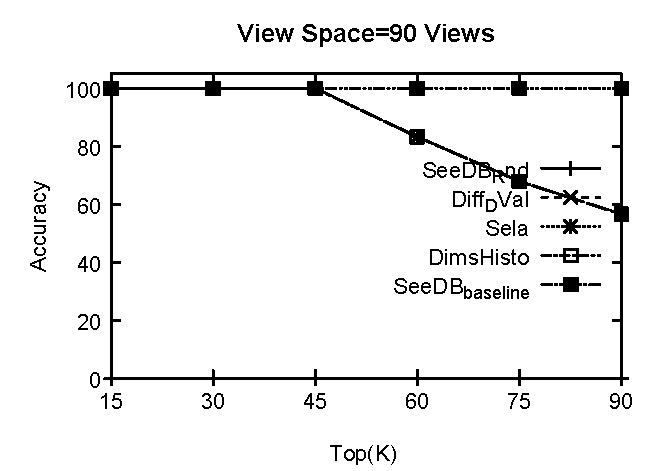
\includegraphics[width=\textwidth]{11.pdf}
%\caption{Accuracy compared with  top(K) views for the Algorithms $Sela$ , $N-N'$, $DimHisto$, and $SeeDB_Rnd$}
%\label{fig:fig3}%
%\end{figure}

\begin{figure}[t]
 \centering
%\end{figure}
  \begin{subfigure}[b]{0.42\textwidth}
    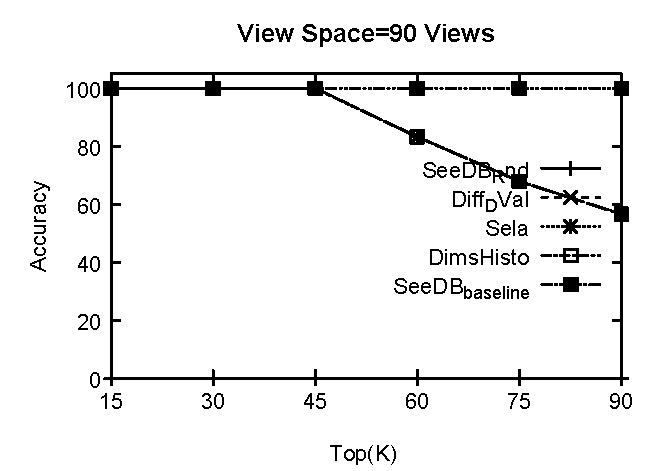
\includegraphics[width=\textwidth]{11.pdf}
    \caption{Accuracy}
       \label{fig:fig3}
  \end{subfigure}
  %
  \begin{subfigure}[b]{0.42\textwidth}
    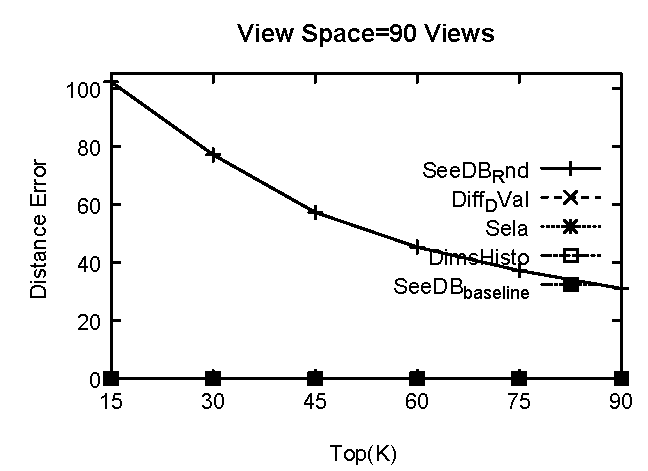
\includegraphics[width=\textwidth]{12.pdf}
     \caption{Distance error}
       \label{fig:fig4}%
  \end{subfigure}
  \caption{Results quality while varying $K$ and $R = 90$}
\end{figure}

Figure \ref{fig:fig3} shows the accuracy of the compared algorithms in a fixed space size $R=90$ while varying $K$. 
%
As shown, all algorithms score \%100 accuracy in the first top 45 views, which form half of the explored views.
%
We observe that the accuracy declines while increasing $K$ in a fixed space limit $R$.
% 
This is because when one dimension attribute is incorrectly prioritized, it will consequently affects all 
recommended views that are created from that dimension attribute. 
%
However, the accuracy is above \%50 when $K=90$ (i.e., the entire view space limit) as shown in Figure \ref{fig:fig3}. 
%
Furthermore, analysts are usually interested in recommending a small number of visualizations, i.e., $K=25$.
%\begin{figure}[t]
%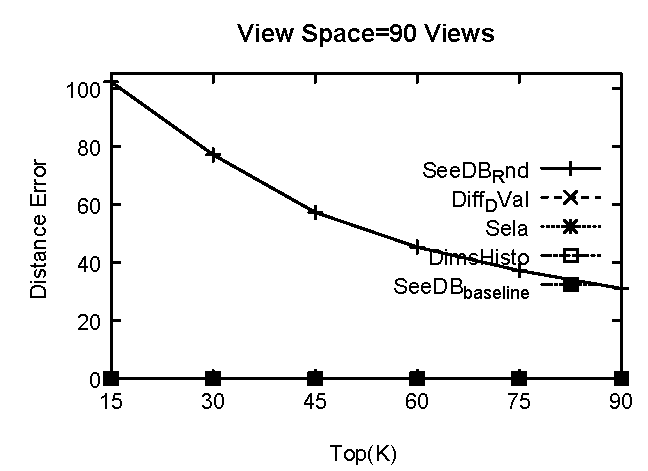
\includegraphics[width=\textwidth]{12.pdf}
%\caption{Error Distance compared with  the view space size for the Algorithms $Sela$ , $N-N'$, $DimHisto$, and $SeeDB_Rnd$}
%\label{fig:fig4}%
%\end{figure}

%\mas{again, what you proposed as better algorithms, performed worse than the basic one, why?!}
In Figure \ref{fig:fig4}, the distance error  of the compared algorithms are shown while varying $K$ and $R$ is fixed to 90 views.
%
All algorithms produce small distance error for $K=60$, however, $Diff DVal$ shows the smallest distance error across different $K$ values. 
%
Both $Sela$  and $DimHisto$ report growing distance error with respect to Top-$K$ required by the analyst in certain view space $R=90$.
%

While the discussed algorithms show high accuracy and low distance errors along different $R$ and $K$ values, as  demonstrated above, these algorithms differentiate on the quality measures.
%
For instance, $Sela$ and $Diff DVal$ obtain higher accuracy when compared with $DimHisto$ as shown in Figures \ref{fig:fig1} and \ref{fig:fig3}, but $Diff DVal$ obtains the lowest distance error, as shown in Figures \ref{fig:figa2} and \ref{fig:fig4}.
 %